\chapter{Experimenty a výsledky}

V této kapitole se podíváme na tři typy experimentů, které s naším systémem
můžeme provádět. Knihovna implementuje několik různých přístupů jak roboty
řídit a jak je vyvíjet pomocí evolučních algoritmů. Následující experimenty
předvedou vzorek z těchto přístupů. 

Cílem všech následujících experimentů je pomocí evolučních algoritmů vyvinout
zvoleného robota tak, aby byl schopný stabilního pohybu v simulovaném prostředí
v předem určeném směru. Kvalita jedinců je pak jednoduše vypočtena dle
následující rovnice:

\begin{equation} \label{fitness_calc}
    fitness = x - 0.5\cdot|y|
\end{equation}

Každý jedinec začíná svůj simulační běh v prostředí v počátku na souřadnicích
$(x,y) = (0,0)$, tedy v rovnici \ref{fitness_calc} jsou $x$ a $y$ vzdálenosti
od počátku, které jedinec v simulovaném prostředí urazil (buď do vypršení
limitovaného času na simulaci, nebo do dosažení podmínky předčasně ukončující
simulační běh -- např. pád robota).

V prvním experimentu v sekci \ref{exp1} se podíváme na ověření, zda pro řízení
jednoduchých robotů nám stačí základní evoluční algoritmy a pro složitější
roboty (s větším množstvím stupňů volnost) potřebujeme pokročilé přístupy.
V následujících dvou experimentech v sekci \ref{exp2} popíšeme experimenty
předvádějící možnost evolučního vývoje jak řízení tak morfologie robotů.

\section{Vývoj řízení robotů} \label{exp1}

\begin{figure}[!htb]
    \centering
    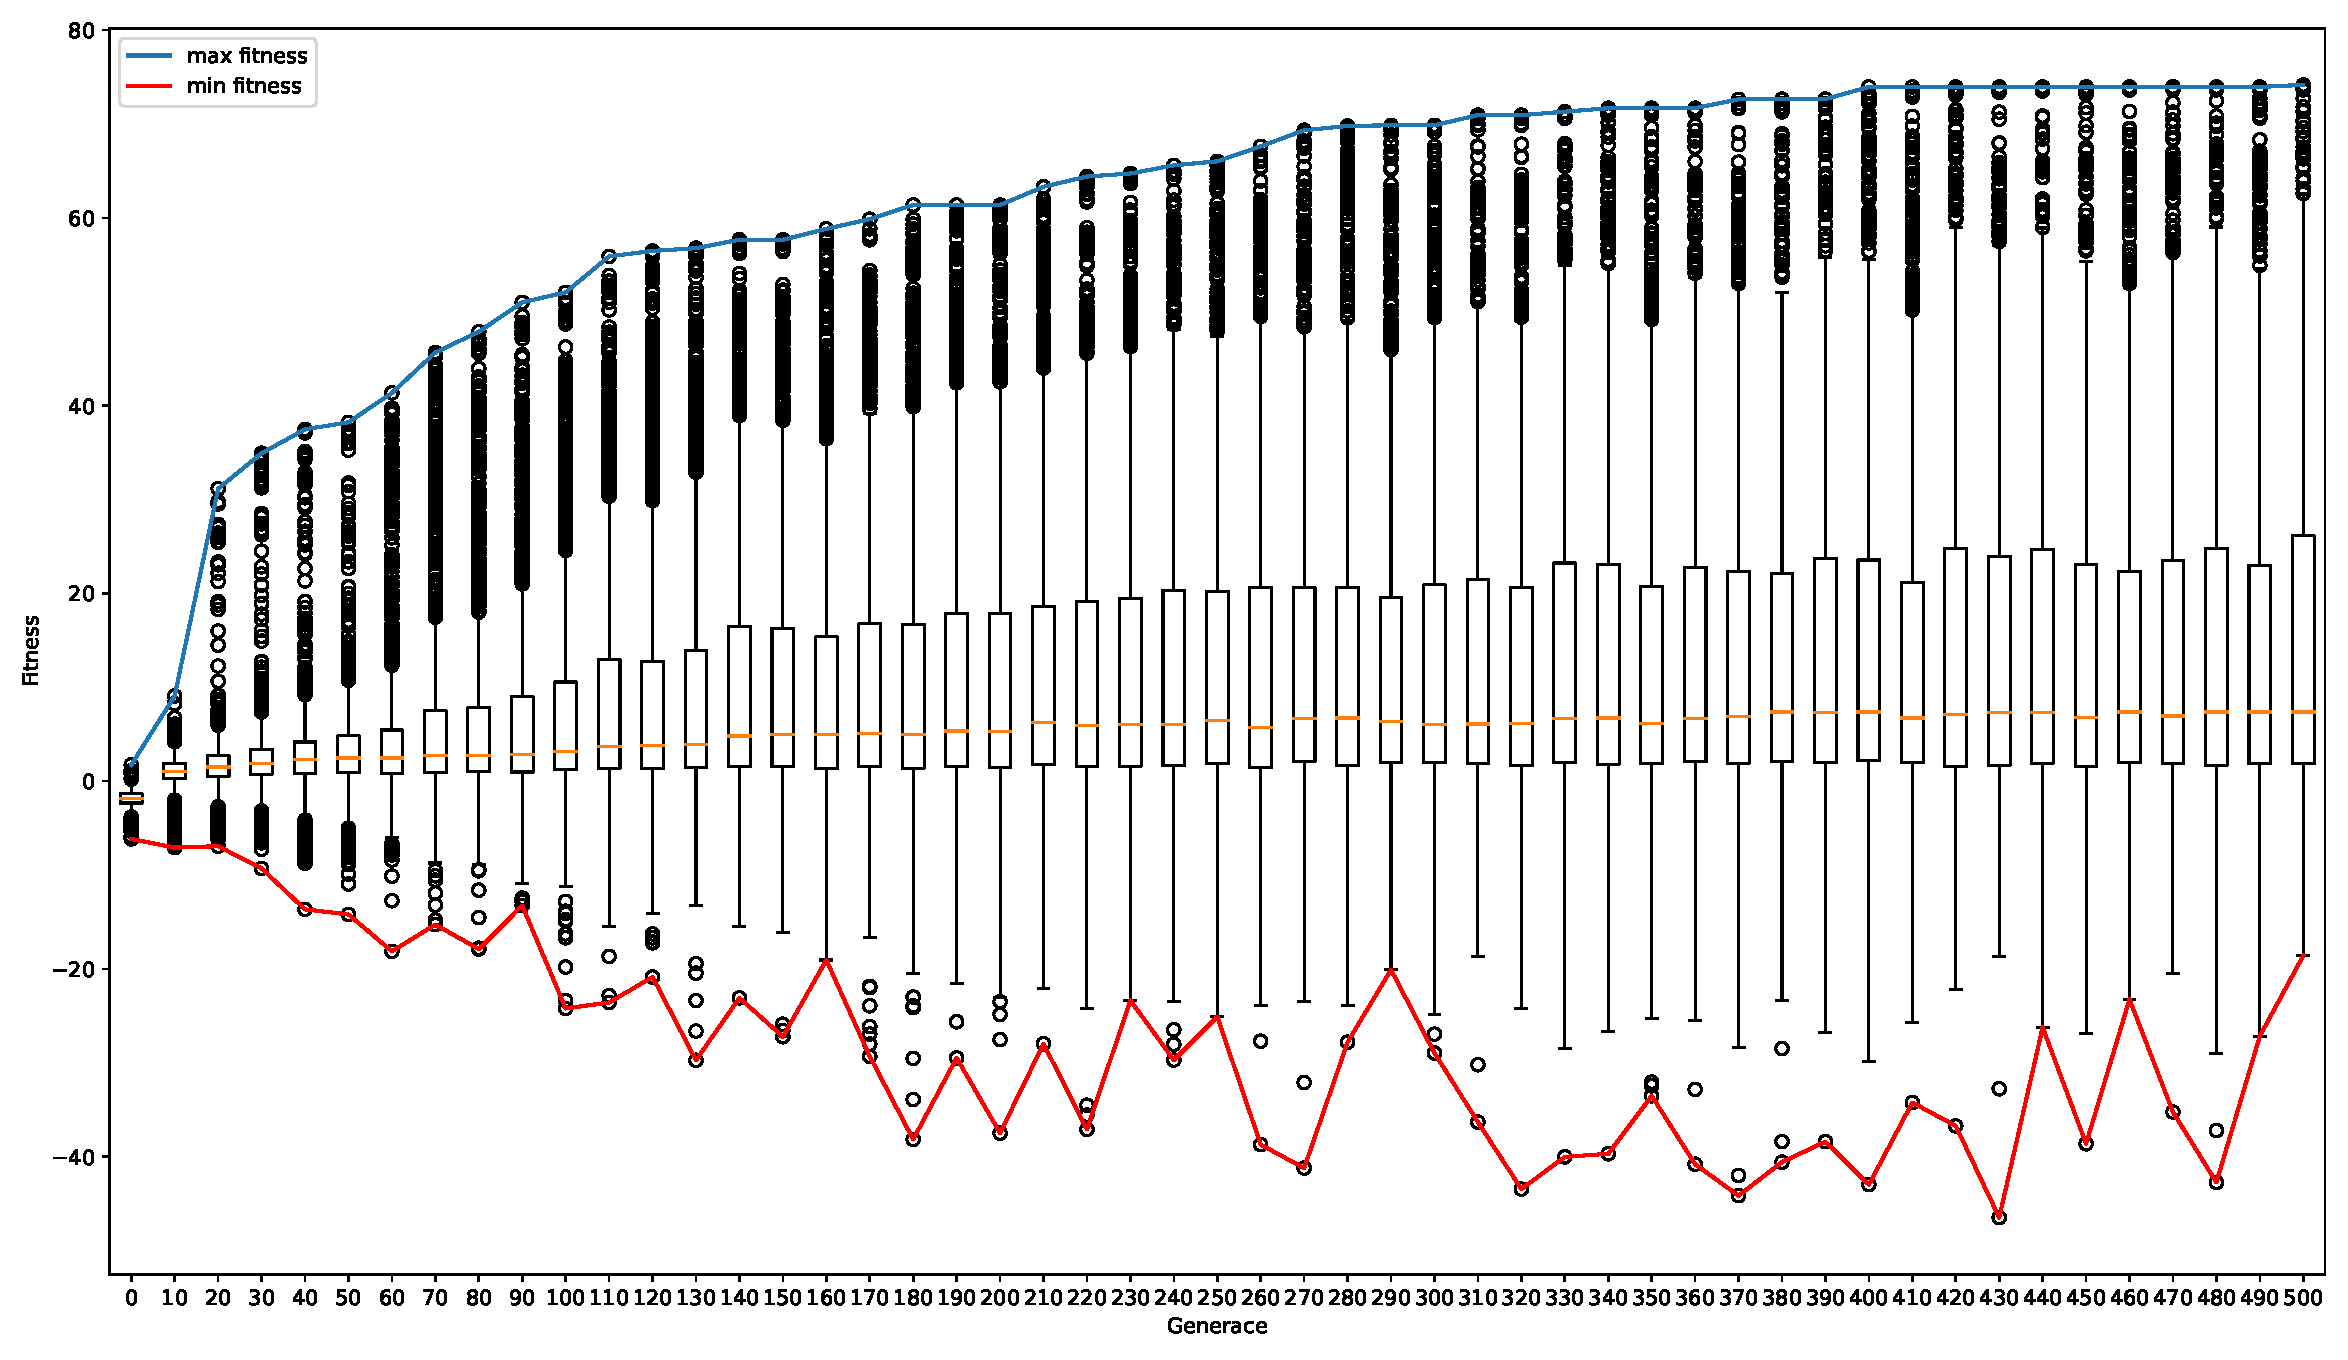
\includegraphics[width=1\textwidth]{../img/BIGexperiment1_TFS_10ticks.pdf}
    \caption{TEST velkého experimentu pro omezení velikosti statistického
    rozboru, 20 opakování algoritmu po 500 generacích}
\end{figure}

\pagebreak
V této sekci se zaměříme na vývoj řízení robotů. Vývoj řízení je ovlivněn
hlavně zvoleným řídícím agentem, který popisuje zvolený evoluční algoritmus.
Tento agent z genetických informací kóduje vstupy pro motory (nastavení kloubů)
robota. Určití agenti mohou využívat přímou reprezentaci vstupů pro motory, kde
sama genetická informace reprezentuje nastavení motorů. Jiní využívají nepřímou
reprezentaci, kde genetické informace slouží jako parametry pro generování
aktuálního nastavení motorů.

\begin{figure}[!htb]
    \centering
    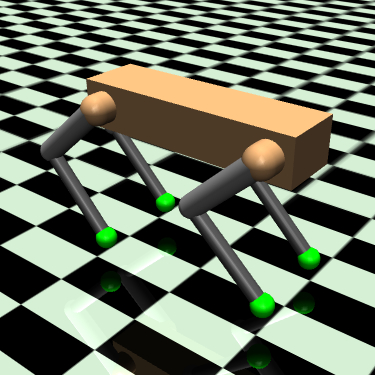
\includegraphics[width=0.4\textwidth]{../img/crop_SpotLike.jpg}
    \caption{Robot \emph{SpotLike}}
    \label{fig:robot:spotlike}
\end{figure}

%TODO: imp ref robots SPOT
První pokus se bude snažit vyvinout řízení pro pokročilého robota v projektu
označovaném jako \emph{SpotLike} (blíže popsaný v implementaci v sekci
\ref{imp:robots.Spot}). Jedná se o robota kráčejícího na čtyřech nohách, kde každá
noha má 3 stupně volnost (tedy 12 celkem pro celého robota). Můžeme ho tedy
řadit mezi roboty, u kterých již bude obtížnější vyvinout stabilní pohyb v
určeném směru.

Kráčení, kterého bychom u robotů chtěli dosáhnout, si můžeme představit jako
poměrně jednoduchý periodický pohyb. Proto se pro vývoj řízení pokusíme využít
agenty, kteří interně podle parametrů generují periodické hodnoty pro motory
robotů. 

\paragraph{}
Nejprve se pokusíme řízení robota vyvinout pomocí evolučního
algoritmu, který kóduje nastavení motorů pomocí základních periodických funkcí
(agent popisující tento algoritmus popsán v implementaci v sekci
\ref{imp:gaAgents.sinefuncfullagent}). Každý motor robota má v tomto případě
přiřazenou vlastní periodickou funkci a genotyp jedinců specifikuje parametry
těchto periodických funkcí (4 parametry pro každý kloub -- amplituda,
frekvence, $x$ a $y$ posun).

Evoluční algoritmus poběží \textbf{200 generací} se \textbf{100} náhodně
inicializovanými jedinci. Pro vyhodnocení bude celý běh evolučního algoritmu
bude pětkrát opakován vždy s novou náhodně vygenerovanou první populací.

\begin{figure}[!h]
    \centering
    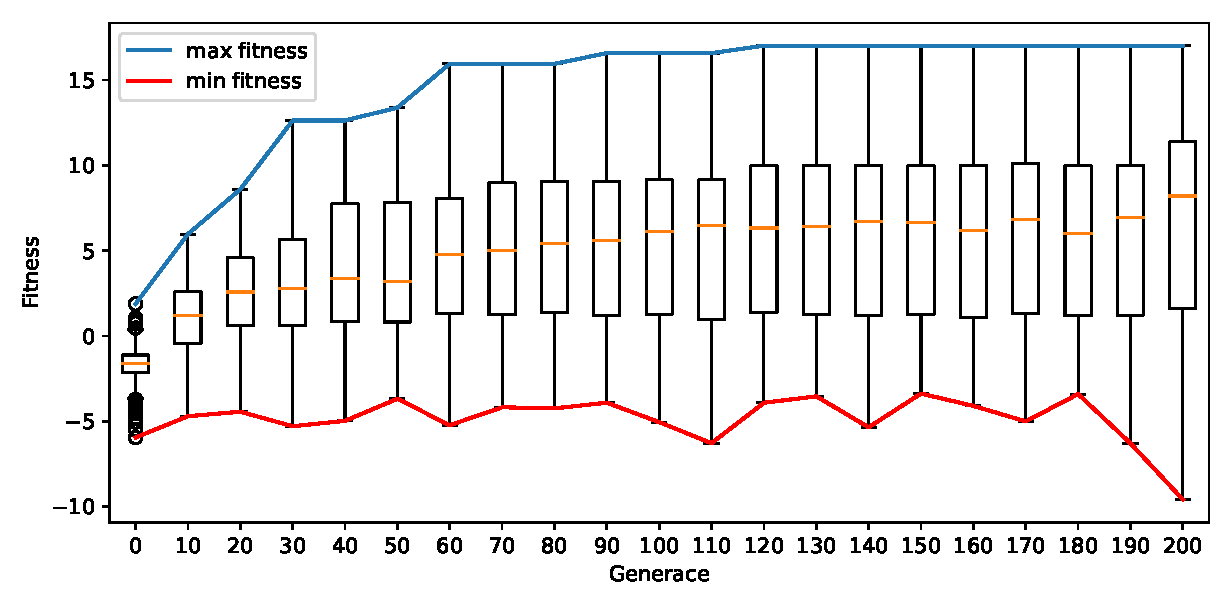
\includegraphics[width=1\textwidth]{../img/experiment1_Sine_10ticks.pdf}
    \caption{Vývoj fitness populace v experimentu se základním agentem}
    \label{exp:first_sinefull}
\end{figure}

Graf na obrázku \ref{exp:first_sinefull} zobrazuje vývoj fitness
hodnot za běhu výše popsaného evolučního algoritmu. Data jsou vytvořena
kombinací záznamů o fitness hodnotách v dané generaci ze všech pěti nezávislých
běhů.

Z grafu se ukazuje, že tento přístup vývoje řízení dosáhl maximální hodnotu
fitness okolo 10 a absolutní většina populace není schopna většího posunu. 

\paragraph{}
Pro porovnání volíme pokročilého agenta, kódujícího nastavení motorů pomocí
omezených Fourierových řad (agent popsán v sekci \ref{imp:gaAgents.TFSagent}).
Tento agent je na úkor malého zvětšení genotypu, oproti předchozímu agentovi
schopný generovat mnohem komplexnější periodické funkce popsané skládáním
několika funkcí sinus.

Stejně jako v předchozím běhu, algoritmus poběží 200 generací se 100 jedinci a
bude opět pětkrát zopakován.

\begin{figure}[!h]
    \centering
    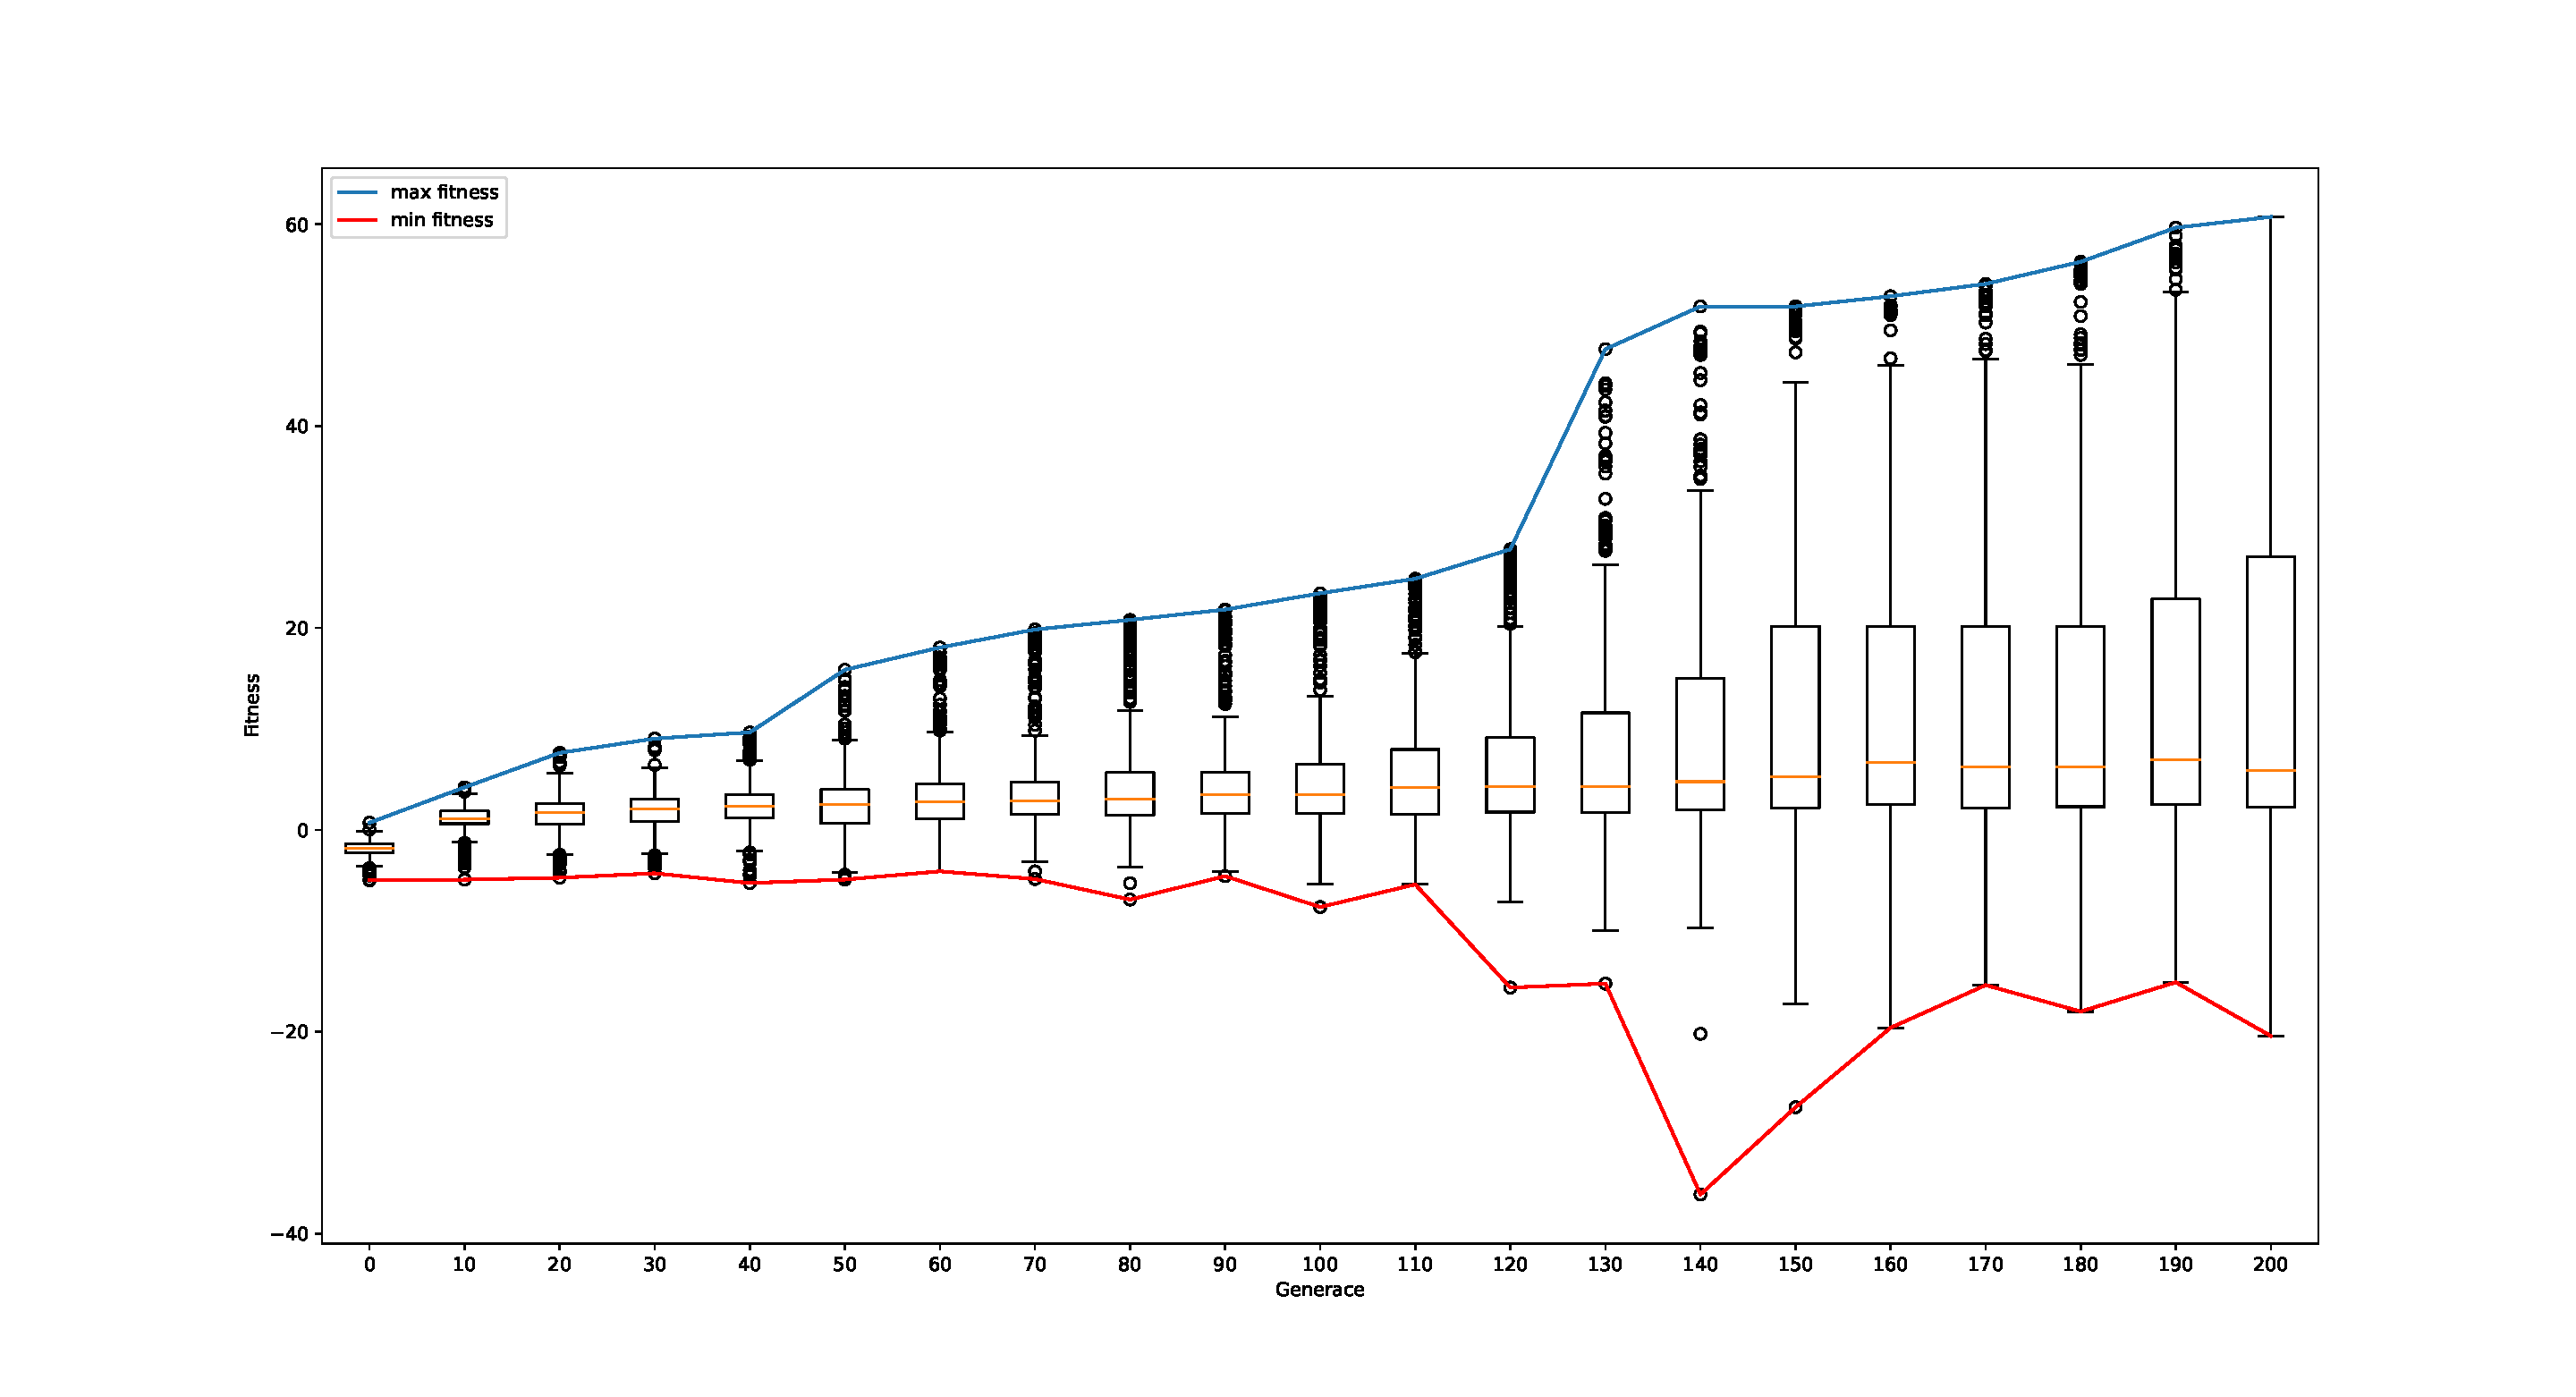
\includegraphics[width=1\textwidth]{../img/experiment1_TFS_10ticks.pdf}
    \caption{Vývoj fitness populace v experimentu s pokročilým agentem}
    \label{exp:first_TFS}
\end{figure}

Graf \ref{exp:first_TFS} vývoje fitness hodnot z experimentu s
pokročilým agentem ukazuje, že tento agent již je schopný vyvinout stabilní
pohyb i pro zadaného komplexního robota. Maximální fitness hodnota, které při
vývoji agent dosáhl se pohybovala okolo 60. Zároveň poměrně velká část populace
byla schopná dosáhnout výsledků, přesahující nejlepší výsledky jednoduššího
agenta. Vývoj fitness dále naznačuje, že pokud bychom navýšili počet generací,
tak by byla možnost pohyb dále optimalizovat a dosáhnout tak ještě vyšší
fitness. 

\paragraph{}
Z experimentů zároveň dostaneme i nejlepšího jedince z poslední generace
evolučního algoritmu. Jelikož naše simulované fyzikální prostředí je
deterministické, můžeme řešení nejlepšího jedince zpětně vizualizovat.

Ruční kontrolou těchto výsledků jsme dále zjistili, že pouze část (dva z pěti
běhů) dosáhly takového pohybu, který bychom od robota této morfologie
očekávali. Tělo v robota v těchto případech (až na menší odchylky) směřovalo
rovně, způsobem připomínající chůzi čtyřnohých zvířat podobné morfologie. Zbylé
běhy vyvinuly pohyb, který je schopný stabilní, ale ne zcela estetické chůze.
Roboti se v těchto případech posouvali stranou, využívající většího rozsahu
v rotaci (\emph{kyčelních}) kloubů pro stabilizaci.

Osobně si myslím, že vývoj estetického pohybu pro tohoto robota je s malou
úpravou hodnotící funkce možný. Ta by například mohla penalizovat rotaci těla
od požadovaného směru pohybu. Chůze stranou je kvůli rozsahu (\emph{kyčelních})
kloubů (hlavně v ose délky těla robota) mnohem snazší na vyvinutí a tak tento
způsob chůze tvoří silné lokální optimum. Agenti velmi rychle konvergují ke
způsobům chůze, které jsou stabilní, což jim navyšuje šanci urazit větší
vzdálenost bez pádu. Chůze stranou je oproti vratké chůzi rovně mnohem
stabilnější. Navržená jednoduchá úprava hodnotící funkce by měla být schopna
toto lokální optimum penalizovat a tedy přinutit estetičtější pohyb.

\paragraph{}
Ve srovnání s předchozími pokusy se nyní pokusíme pomocí vyvinout řízení
jednoduššího robota označeného jako \emph{Ant} (popsán v implementaci v sekci
\ref{imp:robots.Ant}). Můžeme ho brát jako jednoduššího, protože obsahuje menší
počet kloubů (8 stupňů volnosti) v porovnání s robotem \emph{SpotLike}. Zároveň
jeho morfologie umožňuje snazší pohyb všemi směry s menším rizikem pádu.

\begin{figure}[!htb]
    \centering
    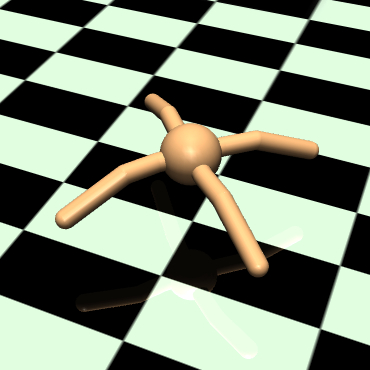
\includegraphics[width=0.4\textwidth]{../img/crop_Ant-v3.jpg}
    \caption{Robot \emph{Ant}}
    \label{fig:robot:ant}
\end{figure}

Řízení se budeme snažit vyvinout pomocí agentů se stejnými parametry jako v
případě s pokročilým robotem. Celý běh bude opět pro statistické vyhodnocení
pětkrát opakován se stejnou velikostí náhodně vygenerované populace
(\textbf{100 jedinců}). Jelikož kvůli menšímu počtu stupňů volnosti očekáváme
schopnost agentů vyvinout řízení rychleji, zkrátíme délku evoluci na
\textbf{100 generací}.

\begin{figure}[h!]
    \centering
    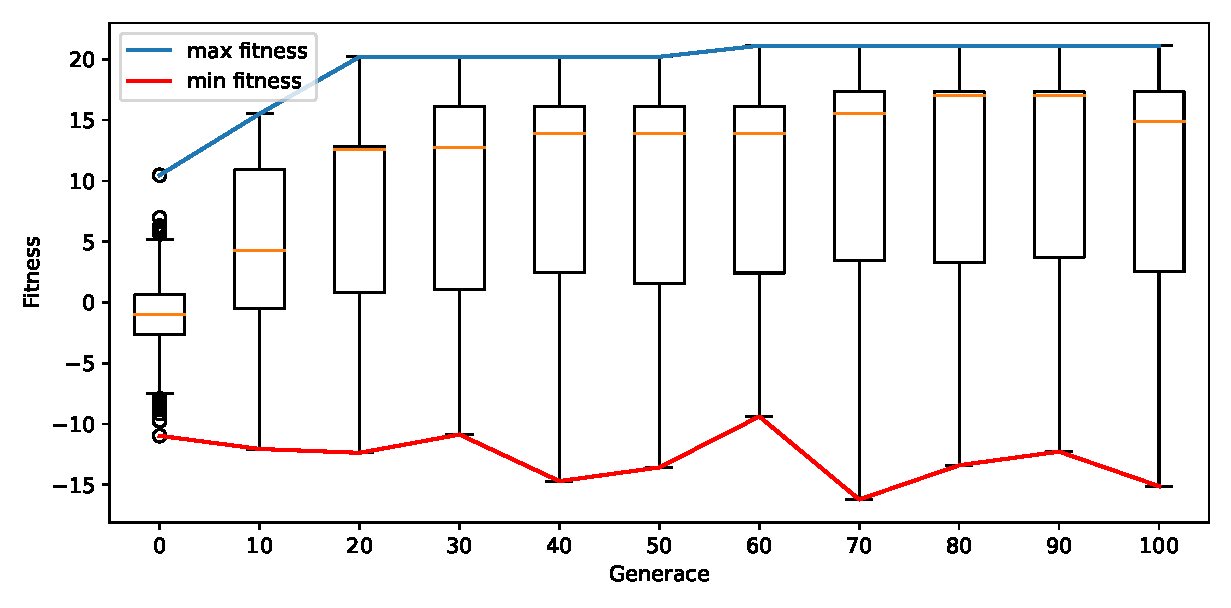
\includegraphics[width=1\textwidth]{../img/experiment1_2_Sine_10ticks.pdf}
    \caption{Vývoj fitness populace se základním agentem a jednodušším robotem}
    \label{exp:first2_sinefull}
\end{figure}
\begin{figure}[h!]
    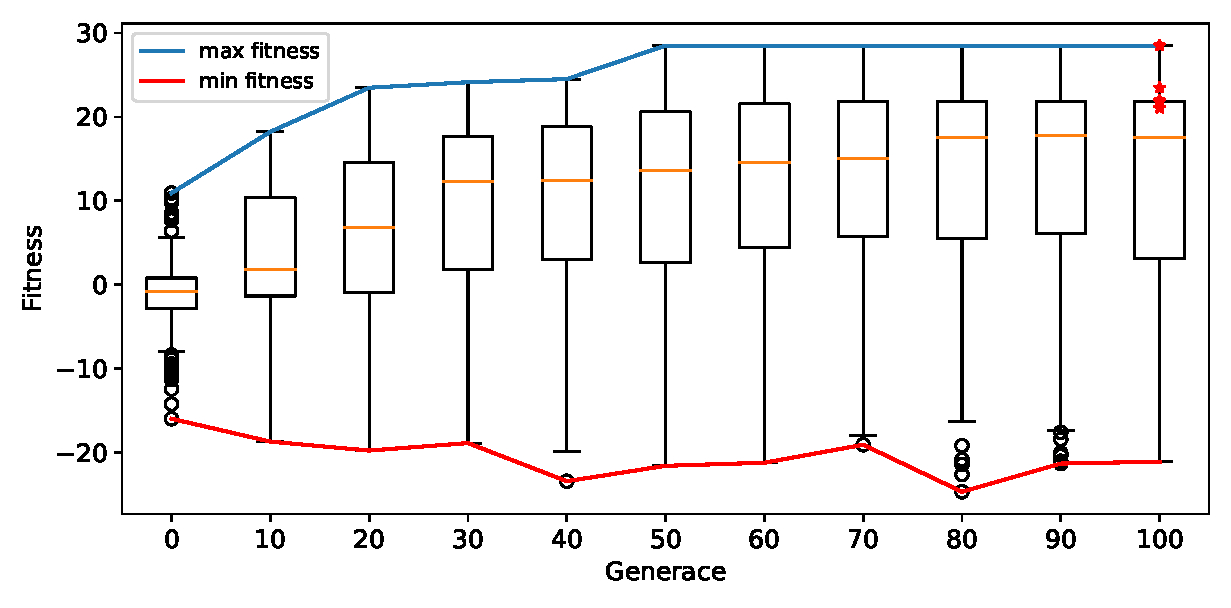
\includegraphics[width=1\textwidth]{../img/experiment1_2_TFS_10ticks.pdf}
    \caption{Vývoj fitness populace s pokročilým agentem a jednodušším robotem}
    \label{exp:first2_TFS}
\end{figure}

\pagebreak
Z vývoje fitness (v grafu \ref{exp:first2_sinefull} a \ref{exp:first2_TFS})
můžeme pozorovat, že oba agenti byli schopní u tohoto jednoduššího robota
dosáhnout přijatelných výsledků i s omezeným počtem generací. Přijatelné
výsledky jsou částečně podpořeny faktem, že i náhodně konfigurace mají dobrou
šanci tohoto robota rozpohybovat v požadovaném směru a tedy již velmi brzy
získat dobré ohodnocení. To se zároveň projevuje i na minimální fitness. Pro
tohoto robota je totiž stejně jednoduché dostat takovou konfiguraci motorů,
které ho rozpohybují v opačném směru (jedinec z definice hodnotící funkce
obdrží záporné ohodnocení).

\section{Vývoj řízení a morfologie robotů} \label{exp2}

V této sekci předvedeme dva další typy experimentů, které naše knihovna
podporuje -- simultánní vývoj (podsekce \ref{exp2:para_evo}) a oddělený
vývoj (podsekce \ref{exp2:split_evo}) řízení a morfologie.

Tyto experimenty se od předchozích liší tím, že evolučnímu algoritmu povolíme
vyvíjet i zvolené části těla robota. To teoreticky umožní z těla původního
robota vyvinout optimálnější morfologii pro zadaný problém.

Vývoj těla je implementací umožněn díky speciálním značkám v XML konfiguračních
souborech (popsaných v konfiguraci vlastního robota v sekci \ref{imp:robots}),
pomocí kterých roboti mohou upravovat konfiguraci svého těla.

\subsection{Simultánní vývoj řízení a morfologie} \label{exp2:para_evo}

V prvním příkladu předvedeme experiment, ve kterém provedeme současný vývoj jak
řízení, tak morfologie těla robota.

Kvalita jedinců bude v tomto experimentu hodnocena stejně jako v předchozích.
Cílem pro jedince je tedy dojít co nejdál v určeném směru. Přesný výpočet
fitness je popsán rovnicí \ref{fitness_calc}. Experiment předvedeme s robotem
\emph{AntV3} (popsán v implementaci v sekci \ref{imp:robots.Ant})

\paragraph{Vývoj robota \emph{AntV3}}
V první ukázce použijeme robota \emph{AntV3} ovládaného agentem
\emph{SineFuncHalfAgent} (popsaného v sekci
\ref{imp:gaAgents.sinefunchalfagent}). \emph{AntV3} je robot se složitější
morfologií nohou, pomocí kterých se pohybuje, a tudíž se hodí pro základní
pokusy s vývojem těla. 

Tento experiment je dostupný v modulu \emph{experiment\_setter} pod názvem
\texttt{exp20\_AntV3}.

%TODO: DATA

% KECI O DATECH

\subsection{Oddělený vývoj řízení a morfologie} \label{exp2:split_evo}

V tomto příkladu předvedeme experiment vyvíjející řízení a morfologii robota,
nicméně tyto části vývoje jsou od sebe oddělené. Doba vývoje se prodlouží, ale
tím jedinci dostanou možnost nejprve vyvinout samotný pohyb (bez změn
morfologie robota) a následně zafixovat pohyb a evolučním vývojem optimalizovat
tělo robota pro specifický pohyb. Tímto přístupem by teoreticky jedinci měli
být schopni dosáhnout lepších výsledků, než při vývoji samotného řízení.

\section{Diskuze výsledků}
